\section{System}
\label{sec:system}
FOI designed the SWIR SPC platform using a DMD, a Newtonian telescope and a single pixel detector which are further described in section~\ref{sec:hardware}. The system also has a reference camera in the visual spectrum  which can capture images if all micro mirrors in the DMD are turned away from the single pixel sensor and towards the reference camera, it can also be used to check that the patterns are displayed correct.  

\begin{figure}[H]
    \centering
    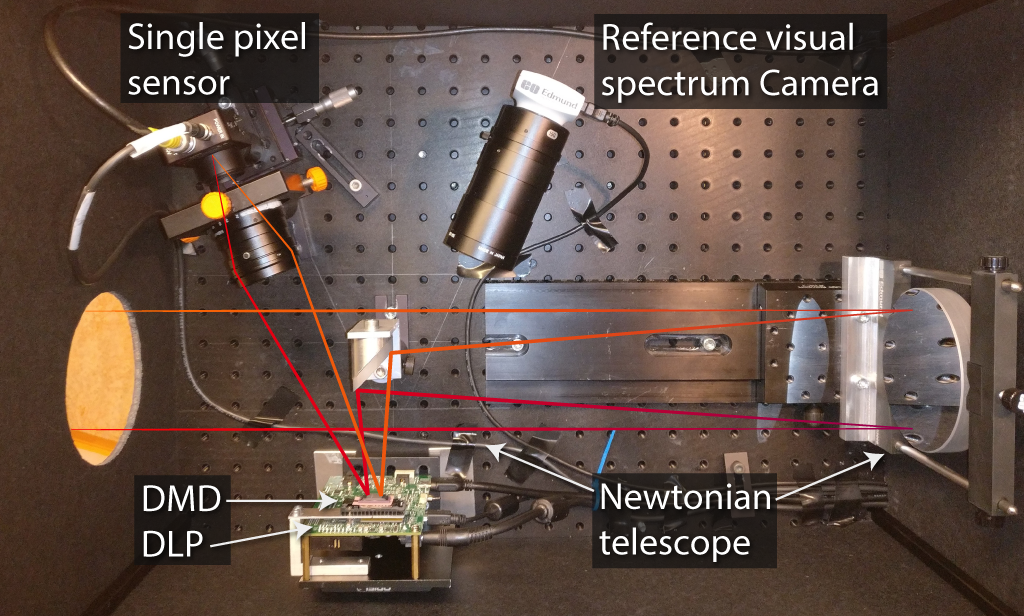
\includegraphics[width = 0.8\textwidth]{gfx/SPC.png}
    \caption{Single pixel imaging system (SPIS), adopted from \cite{article:foiSPIS}.}
    \label{fig:system1}
\end{figure}



As seen in figure~\ref{fig:system1} light from the scene is focused by the Newtonian telescope and reflected onto the DMD. The mirrors on the DMD can turned individually either into the single pixel sensor or the reference camera. The DMD acts as a Spatial Light Modulator (SLM) and reflects different patterns which is 'summed up' in the single pixel sensor as an intensity. The reconstructed image from the system will have the same resolution as the DMD patterns. The DLP is the DMD control unit which controls which patterns that are displayed on the DMD either by reading images from memory or the video port.   

\subsection{Hardware}
\label{sec:hardware}
\subsubsection{Newtonian telescope}
A Newtonian telescope is a reflecting telescope, using a concave primary mirror and a flat diagonal secondary mirror, see figure~\ref{fig:system1}. In this set-up the telescope act as a lens focusing the scene onto the DMD. The motivation to use a Newtonian telescope instead of a lens system is partly that chromatic aberration is eliminated and partly that a reflective optical system works over a greater range of wavelengths that includes SWIR, near infrared (NIR) and the visible spectrum.

\subsubsection{DLP and DMD}
>>>> Skriv om hela stycket, Beskriv att DLP är kontrollenheten och att den läsen en vanlig signal där videosignalens alla bitplan kan avläsas. I detta examensarbetet är inte hastighet en prioritet därför läggs uppdateringen av patterns på 90 Hz.<<<<

The DMD (Texas Instruments DLP4500NIR) is a matrix of micro mirrors that can be individually tilted $\pm 12^{\circ}$ and reflects wavelengths in the range 700-2500 nm. The DMD is controlled by the DLP (DLP LightCrafter 4500) which can be controlled either by video port (HDMI) or by the internal flash memory. 

The video port can be operated at 120 Hz while the internal storage in pattern mode can be operated in 250-300 Hz at maximum. The constraint while operating the DMD in pattern mode is that the flash memory only can hold 1536 patterns. For larger resolutions that requires more then 1536 patterns, slower capturing with the video port is used in 90-180 Hz. 


Because the diamond shape of the mirrors and how their index is defined in the DLP where one column is two mirror column arrays wide, see figure~\ref{fig:dmd_index}, the reconstructed image needs to be reshaped to a Cartesian grid. To control the DMD the software 'DLP LightCrafter 4500 Control Software' is used. \cite{manual:DLP}

>>>> Beskriv hur det nya mönstret ser ut <<<<


\begin{figure}[H]
    \centering
    
\includegraphics[width = 0.8\textwidth]{gfx/DMD_grid.png}
    \caption{DMD matrix, left shows each tiles index and right shows second row and second column in black.}
    \label{fig:dmd_index}
\end{figure}

\begin{figure}[H]
    \centering
    
\includegraphics[width = 0.8\textwidth]{gfx/DMD_grid2.png}
    \caption{DMD matrix, left shows each tiles index and right shows second row and second column in black.}
    \label{fig:dmd_index2}
\end{figure}


\subsubsection{Lens}
The lens mounted on the single pixel sensor is an 50mm SWIR Fixed Focal Length Lens f1.4 designed for wavelengths raging from the 800 nm in the visual spectrum to 2000 nm in the SWIR spectrum. \cite{website:SWIR_objective}

\subsubsection{Single pixel sensor}
The single pixel sensor is a Thorlabs PDA20C/M and is sensitive in wavelength range 800-1700 nm which is beyond the visual spectrum (390-700 nm). \cite{manual:PDA}

\subsubsection{Signal spectrum}
All components characteristics assembled should capture signals in 800-1700 nm spectrum.











